\chapter*{Week 3: Booleans and Conditions}
\addcontentsline{toc}{chapter}{Week 3: Booleans and Conditions}
\setcounter{chapter}{3}
\setcounter{section}{0}

\begin{abstract}
This week you will:
\begin{enumerate}
    \item Understand the Boolean data type and boolean operators
    \item Understand relational operators
    \item Be able to implement decisions using if statements

\end{enumerate}
    
\end{abstract}

\section{Background}

\subsection{Booleans}
Booleans are a special data type that stores only ``true" or ``false". This true or false value can be stored in a boolean variable, or it can be the result of evaluating different expressions.

\subsubsection{Relational Operators}
A relational operator is a feature of a programming language that tests or defines some kind of relation between two entities. These include numerical equality (e.g., \mintinline{c++}{5 == 5}) and inequalities (e.g., $4 \geq 3$). Relational operators will evaluate to either True or False based on whether the relation between the two operands holds or not. When two variables or values are compared using a relational operator, the resulting expression is an example of a boolean condition that can be used to create branches in the execution of the program. Below is a table with each relational operator’s C++ symbol, definition, and an example of its execution.

\begin{table}[H]
    \centering
    \begin{tabular}{c|c|c}
        Operator & Meaning & Example \\ \hline
        $>$ & greater than & $5 > 4$ is TRUE \\
        $<$ & less than & $4 < 5$ is TRUE \\
        $>=$ & greater than or equal & $4 >= 4$ is TRUE \\
        $<=$ & less than or equal & $3 <= 4$ is TRUE \\
        == & equal to & $5 == 5$ is TRUE \\
        != & not equal to & $5 != 6$ is TRUE
    \end{tabular}
\end{table}

\subsubsection{Logical Operators}
Logical operators are used to compare the results of two or more conditional statements, allowing you to combine relational operators to create more complex comparisons. Similar to relational operators, logical operators will evaluate to True or False based on whether the given rule holds for the operands. Below are some examples of logical operators and their definitions.

\begin{table}[H]
    \centering
    \begin{tabular}{c|c|c}
    \mintinline{c++}{&&} & AND & returns true if and only if both operands are true\\
    \mintinline{c++}{||} & OR & returns true if one or both operands are true \\
    ! & NOT & returns true if the operand is false and false if the operand is true
    \end{tabular}
\end{table}

Every logical operator will have a corresponding truth table, which specifies the output that will be produced by that operator on any given set of valid inputs. Below are truth tables for each of the logical operators specified above.

AND ( \mintinline{c++}{&&} ): These operators return true if and only if both operands are True. This can be visualized as a venn diagram where the circles are overlapping.

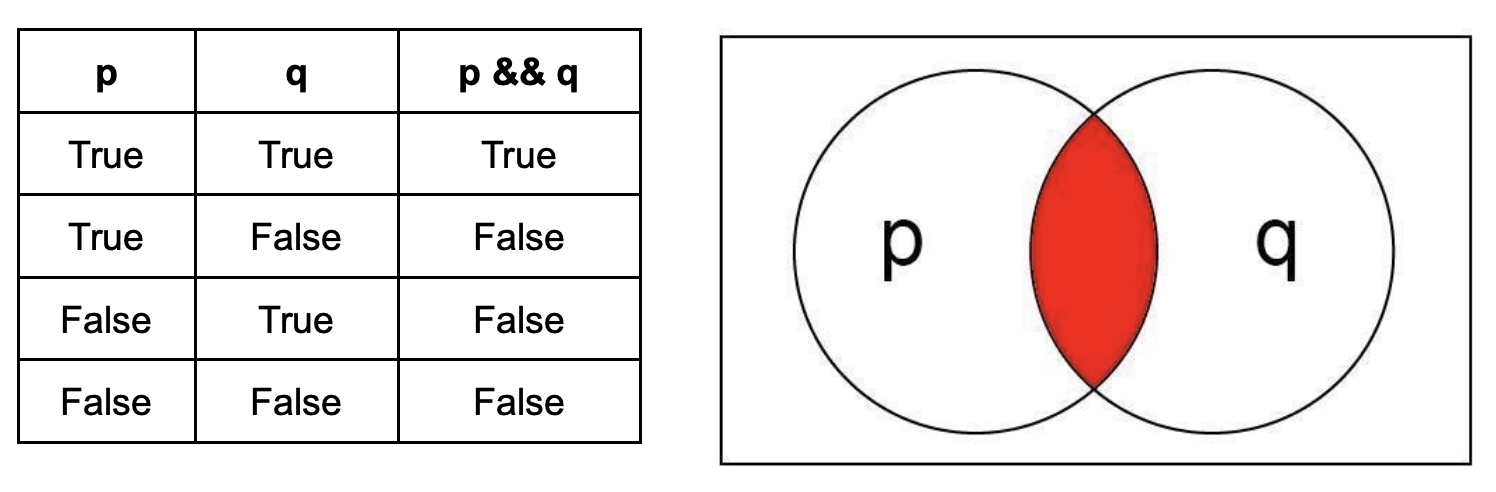
\includegraphics[width=\textwidth]{images/and.png}

OR ( \mintinline{c++}{||} ): These operators return True if one or both of the operands are True. This can be visualized as the region of a venn diagram encapsulated by both circles.

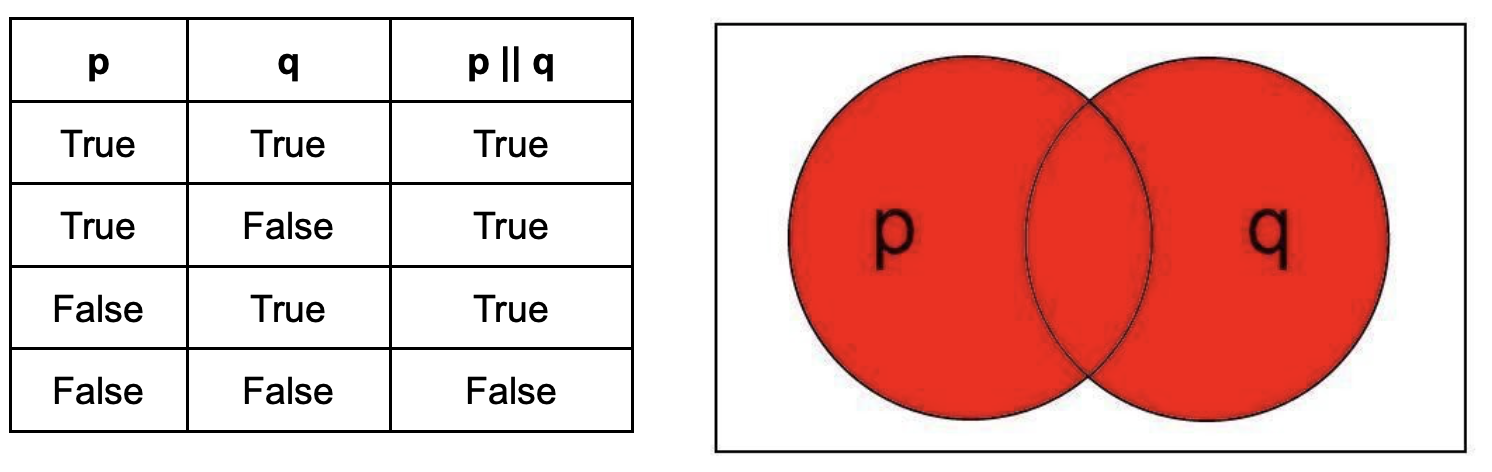
\includegraphics[width=\textwidth]{images/or.png}

NOT ( ! ): This operator returns the opposite of the operand. This can be visualized as the region of a venn diagram outside the circle. Unlike AND and OR, the NOT operator has only one operand.

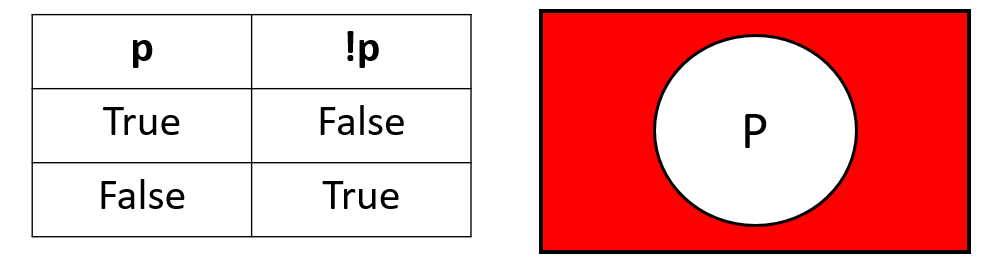
\includegraphics[width=\textwidth]{images/not.png}

You can create truth tables for more complicated expressions by combining elements of these tables. You should begin with columns of the basic variables representing each possible combination of those variables, and then add columns to represent their modified values. For example, if you wanted to create a truth table for \mintinline{c++}{!p && q} you could make a column for \mintinline{c++}{p} and a column for \mintinline{c++}{q} representing all possible combinations of true/false between the two variables. You can then create a third column for \mintinline{c++}{!p}, and then perform the \mintinline{c++}{&&} operation between the \mintinline{c++}{!p} and \mintinline{c++}{q} columns instead of the \mintinline{c++}{p} and \mintinline{c++}{q} columns, like this below:

\begin{table}[H]
    \centering
    \begin{tabular}{c|c|c|c}
        \mintinline{c++}{p} & \mintinline{c++}{q} & \mintinline{c++}{!p} & \mintinline{c++}{!p && q} \\ \hline
        True & True & False & False \\
        True & False & False & False \\
        False & True & True & True \\
        False & False & True & False
    \end{tabular}
\end{table}

For simple expressions, you can often work through the truth table in your head. However, knowing how to make truth tables will be helpful when you need more complicated expressions.

\subsubsection{Using Booleans}
There are two main ways you can use booleans: you can either assign them to a boolean variable, or you can use them directly as a condition (such as in an if statement). If you would like to evaluate a boolean expression and store it in a variable, you can do it like this:

\begin{minted}{c++}
    bool myNewBoolean = (4 < 5); // this will evaluate to true
    bool mySecondBoolean = (5 == 6); //this will evaluate to false
    bool myFinalBoolean = (myNewBoolean && mySecondBoolean); //this will evaluate to false
\end{minted}

You can string together increasingly complicated boolean equations either as a combination of boolean variables or as a combination of relational/logical expressions.

Booleans can also be represented using integers, and will print that way by default in C++. As an integer representation, 0 is false and 1 is true. 

You can build if statements using boolean variables or boolean expressions.

\subsection{Conditionals}
Conditional statements, also known as decision statements or branching statements, are used to make a decision based on condition. A condition is an expression that evaluates to a boolean value, either true or false. \href{https://cal-linux.com/tutorials/conditionals.html}{\textcolor{cyan}{Conditional Execution in C++}} is a good online resource for learning about conditionals in C++.

You have seen one type of conditional expression already: switch statements. If statements, If/Else statements, and If/Else If/Else statements are a more complicated but also more dynamic way to make decisions in your code.

\subsubsection{IF Statements} 

An if statement in C++ is composed of a condition and a body. The body is executed only if the condition is true. The condition appears inside a set of parentheses following the keyword “if” and the body appears within a set of curly brackets after the condition:

The general format for if statements is:

\begin{minted}{c++}
if ( <CONDITION> ){
    <BODY>
}    
\end{minted}

It is good practice to vertically align the closing curly bracket with the start of the if statement, and to indent the body.

The condition is interpreted as a boolean value, either true or false. Be careful, most expressions in C++ have a boolean interpretation. For instance, non-zero numeric values are true. Assignment operations (single equal sign) are interpreted as true as well. A common mistake is to use a single equals sign inside a condition when a double equals sign is intended.

\begin{example}
    Here is an if statement that will check if a number is negative and change it to positive (i.e., find the absolute value):

    \begin{minted}{c++}
if (num < 0){
    cout << "Changing sign" << endl;
    num = -1 * num;
}
    \end{minted}
\end{example}

\subsubsection{IF-ELSE Statements}
 If statements may be paired with else statements in C++. If the condition associated with the if statement is false, the body associated with the else statement is executed. The else statement body is enclosed in a set of curly brackets:

 \begin{minted}{c++}
 if ( <CONDITION> ){
    <BODY>
    // executed when CONDITION is true
}
else{
    <BODY>
    // executed when CONDITION is false
}
 \end{minted}

 An if statement does not need an else statement, but there must be an if statement before every else statement.

 \begin{example}
     Here is an if/else statement that will check if a number can be a divisor before performing division:
     \begin{minted}{c++}
if (num == 0) //notice the double equals!{
    cout << "Can't divide by 0!" << endl;
}
else{
    num = 1000 / num; //integer arithmetic
}         
     \end{minted}
 \end{example}

 \subsection{ELSE-IF Statements}
 
 Finally, an if statement may also be associated with any number of else-if statements. These statements each have an associated condition and an associated body. The body is executed if the condition is true and the conditions for all preceding if- and else-if statements in the same group are false. An else statement may be included at the end of the group but is not required. The else statement will be executed if all the previous conditions are false.

\begin{minted}{c++}
if ( <CONDITION> ){
    <BODY>
}
else if ( <CONDITION> ){
    <BODY>
}
else if ( <CONDITION> ){
    <BODY>
}
else{
    <BODY>
}
 \end{minted}

 This is \textbf{not} logically the same as having multiple sequential if statements. 

 \begin{example}
     These two if statements:
     \begin{minted}{c++}
         if ( <CONDITION A>){
            //do X
         }
         if ( <CONDITION B>){
            //do Y
         }
     \end{minted}
     are NOT logically the same as this if/else-if statement:
     \begin{minted}{c++}
         if( <CONDITION A>){
            //do X
         }
         else if ( <CONDITION B>){
            //do Y
         }
     \end{minted}
 \end{example}

 In the first code section, both if statements are evaluated. If both CONDITION A and CONDITION B are true, we will do \textbf{both} X and Y. Meanwhile, in the second code block, if CONDITION A is true we will never evaluate CONDITION B, and therefore never do execute that code; here, we will \textbf{only} do X. Therefore, we need to use ``else if" only when we want the two conditions to be mutually exclusive.

 \begin{example}
     Here is an if/else if/else statement to tell you if a number is positive, 0, or negative:
\begin{minted}{c++}
if ( num > 0 ){
    cout << "Positive" << endl;
}
else if ( num == 0 ){
    cout << "Zero" << endl;
}
else{
    cout << "Negative" << endl;
}
\end{minted}
 \end{example}

 \subsubsection{Nested If Statements}
 You can put if statements inside of other if statements (or if/else, or if/else if/else). The meaning of logical expressions can change when you are nesting if statements, so you should think through the truth tables for your if/else statements carefully. 

 \begin{minted}{c++}
     if (booleanExpression1){
        //anything here will evaluate if booleanExpression1 is true
        if (booleanExpression2){
            //we will only evaluate this if statement if booleanExpression1 is true, 
            //and then will only execute this statement if booleanExpression2 is ALSO true
        }
     }
 \end{minted}

 Nested if statements are essentially performing a logical ``AND" operation on the two boolean expressions for the innermost if statement, but if only the first if statement is true you can still do other things. 

\subsection{Common Errors}
Unintended behavior when accidentally using assignment operation (= instead of ==) in conditional statements:

\begin{example}
    Here is some (incorrect) code:

    \begin{minted}{c++}
    int x = 5;
    if (x = 1){ // one equal sign: changes value of x, will always evaluate to true
    
        cout << "The condition is true." << endl;
    }
    cout << "x is equal to " << x << endl;
    \end{minted}
    The output of this would look like this:
    \begin{sample}
The condition is true.

x is equal to 1
    \end{sample}
    What you would ACTUALLY want is:
    \begin{minted}{c++}
    // CORRECT CODE
    int x = 5;
    if (x == 1) // two equal signs, performs comparison
    {
        cout << "The condition is true." << endl;
    }
    cout << "x is equal to " << x << endl;
    \end{minted}
    Which would output:
    \begin{sample}
x is equal to 5
    \end{sample}
\end{example}

Remember, ``=" is for assignment and ``==" is for checking equality.

\section{PreQuiz}

\begin{problem}
    What is the difference between arithmetic and relational operators?
\end{problem}

\vspace{4cm}

\begin{problem}
    What is the correct way to write a condition to determine if a variable \mintinline{c++}{num} stores a number between 0 and 4, inclusive?
\end{problem}

\vspace{4cm}

\begin{problem}
    Fill in the blank in the code below with a condition that accounts for temperature in range of 25 (exclusive) to 50 (inclusive) degrees:
\end{problem}

\begin{minted}{c++}
#include <iostream>
using namespace std;

int main()
{
    int temperature = 50;

    if (temperature > 85) {
        cout << "It's a hot day!";
    }
    if (temperature <= 85 && temperature > 50){ 
        cout << "It's a pleasant day.";
    }
    else if (____________________________________________________) { //FILL IN THIS LINE
        cout << "It's a cool day.";
    }
    else {
        cout << "It's a cold day.";
    }

    return 0;
}
\end{minted}

\begin{problem}
    Complete the following truth table to evaluate the expressions for (a \&\& !b).
\end{problem}

\begin{table}[H]
    \centering
    \begin{tabular}{c|c|c|c}
         a & b & !b & a \&\& !b \\ \hline
         T & T &  &  \\
         T & F &  &  \\
         F & T &  &  \\
         F & F &  &  \\
    \end{tabular}
\end{table}

\begin{problem}
    Complete the following truth table to evaluate the expressions for (a || (!a \&\& b)).
\end{problem}

\begin{table}[H]
    \centering
    \begin{tabular}{c|c|c|c|c}
         a & b & !a & !a \&\& b & a || (!a \&\& b)\\ \hline
         T & T &  &  &  \\
         T & F &  &  &  \\
         F & T &  &  &  \\
         F & F &  &  &  \\
    \end{tabular}
\end{table}

\section{Recitation}

\subsection{Spot The Error}

\begin{multipart}
The code snippet below is supposed to determine if a variable stores a value that is greater than, less than, or equal to 8. Identify the error(s) in the code below, and write the correct line(s).
\end{multipart}

\begin{minted}{c++}
#include <iostream>
using namespace std;

int main()
{
    int num = 6;

    if (num > 8) {
        cout << "The number is greater than 8." ;
    }
    else if (num = 8) {
        cout << "The number is equal to 8."; 
    }
    else {
        cout << "The number is less than 8.";
    }

    return 0; 
}
\end{minted}

\begin{multipart}
The code snippet below is supposed to determine if a variable stores a value for an angle that is obtuse, right, or acute. Identify the error(s) in the code below, and write the correct line(s).
\end{multipart}

\begin{minted}{c++}
#include <iostream>
using namespace std;

int main()
{
    int angle = 120;
    if (x>90) { 
        cout<<"It is an obtuse angle." ;
    }
    elif(x=90) {
        cout<<"It is a right angle.";
    }
    else{
        cout<<"It is an acute angle.";
    }
}
\end{minted}

\begin{multipart}
    The code snippet below is supposed to determine if a variable stores a value that is equal to zero or not. Identify the error(s) in the code below, and write the correct line(s).
\end{multipart}

\begin{minted}{c++}
#include <iostream>
using namespace std;

int main()
{
    int num = 7;

    if (num) { 
        cout << "The number is zero.";
    }
    else {
        cout << "The number is not zero.";
    }

    return 0; 
}
\end{minted}

\begin{multipart}
    The code snippet below is supposed to determine if a variable stores a value that is equal to zero or not. Identify the error(s) in the code below, and write the correct line(s).
\end{multipart}

\begin{minted}{c++}
#include <iostream>
using namespace std;

int main()
{
    int num = 0;

    else {
        cout << "This is the 'else' block.";
    }
    if (num == 0) {
        cout << "The number is zero.";
    }
    else {
        cout << "The number is not zero.";
    }

    return 0; 
}
\end{minted}

\begin{multipart}
The following code snippet is expected to accept a user provided integer and then state whether that number is even or odd. Identify the error(s) in the code below, and write the correct line(s).
\end{multipart}

\begin{minted}{c++}
 #include <iostream>
 using namespace std;
 
 int main()
 {
     int num;
     cout << "Provide an integer:" << endl;
     cin >> num;

     if (num/2){
         cout << "The number is even." << endl;
     }
     else {
         cout << "The number is odd." << endl;
     }
 
     return 0; 
 }
\end{minted}

\begin{multipart}
    The following code snippet is expected to accept a user provided character and then state whether the corresponding grade passes or not. Identify the error(s) in the code below, and write the correct line(s).
\end{multipart}

\begin{minted}{c++}
 #include <iostream>
 using namespace std;
 
 int main()
 {
     char grade;
     cout << "Provide a grade (A, B, C, D, or F):" << endl;
     cin >> grade;

     if (grade == 'A' || 'B' || 'C'){
         cout << "This is a passing grade." << endl;
     }
     else if (grade == 'D'){
         cout << "This grade passes with conditions." << endl;
     }
     else {
         cout << "This is a failing grade." << endl;
     }
 
     return 0; 
 }
\end{minted}


\subsection{Step Tracking App}
Your goal is to walk 10,000 steps every day but you aren't great at remembering to do it! So you decide to create a step tracking app that tracks your steps every day and will alert you based on how much you walked for the day. The program first asks how many steps you walked that day and then displays a message based on whether you have hit your goal for the day. Next, it will also tell you how many steps you have left to walk.

The following are the possible messages you will get based on your intake:

\begin{itemize}
    \item If you've walked 5,000 steps or less, then you get: 
    
    \mintinline{text}{You have not walked much today! Get those steps in! You have X steps left to walk.}
    
    \item If you’ve walked more than 5,000 steps but less than 10,000 steps, you get: 
    
    \mintinline{text}{You're doing great, over half way there! You still have X steps left to walk.}

    \item If you've walked 10,000 steps or more, you get:
    
    \mintinline{text}{You've hit your goal for the day! Great job getting exercise!}
\end{itemize}

Note that \textbf{X} is the amount of steps left after subtracting how far you have walked. 

Here is a sample run:

\begin{sample}
How many steps have you taken today?

\textcolor{red}{3000}

You have not walked much today! Get those steps in! You have 7000 steps left to walk.
\end{sample}

\begin{multipart}
    Write an algorithm in pseudocode for the program above.
\end{multipart}

\vspace{4cm}

\begin{multipart}
     Imagine how a sample run of your program would look like. Write at least two examples.
\end{multipart}

\vspace{4cm}

\begin{multipart}
    Identify the values that you must test for. We call these values ``boundary conditions".
\end{multipart}

\vspace{4cm}

\begin{multipart}
    Implement your solution in C++ using VS Code. Revise your solution, save, compile and run it again. Are you getting the expected result and output? Keep revising until you do. Make you sure you test for the values used in your sample runs, and for the boundary conditions. 
\end{multipart}

\section{Homework}

\subsection{Should you charge your phone?}

You are planning to go out with your friends for a hangout. Write a C++ program to determine whether you need to charge your phone further or not based on the current battery level.\\

The program should ask the user to enter their current battery level. If the entered battery level is above 70\% then it should display "You're good to go, you have enough charge" and then terminate. Otherwise, if the entered battery level is below 70\% then it should display "You need to charge your phone" and then terminate.\\ 


Additionally, the program should perform input validation. If the user inputs a non-positive value for battery level (i.e., 0 or a negative number), the program should display "Invalid battery level" and terminate.

\begin{sample} What is your battery level?

\textcolor{red}{78}

You're good to go, you have enough charge \end{sample}

\begin{sample} What is your battery level?

\textcolor{red}{24}

You need to charge your phone \end{sample}

\begin{sample} What is your battery level?

\textcolor{red}{-5}

Invalid battery level \end{sample}


\subsection{TV Subscription}

You've decided to get a new TV. You need to have a TV subscription to watch anything on the TV. You have 3 different kind of plans to choose from: Kids, Teens, Parents. Each plan has a different base price and price per additional channel. The prices are indicated in the table below. Create a program to calculate the total cost of your TV plan. The program should prompt you the name of your plan and the number of additional channels you want and then output the total cost of your TV plan.


\begin{table}[H]
    \centering
    \begin{tabular}{c|c|c}
        Plan Name & Base Price & Price Per Additional Channel \\
        K & 10.00 & 1.50 \\
        T & 12.00 & 2.75 \\
        P & 16.00 & 4.25
    \end{tabular}
\end{table}

The input should be a character (for plan name) and a non-negative integer (for the number of additional channels). The program should accept both lowercase and uppercase inputs for pizza sizes (e.g., `k', `t', `p' or `K', `T', `P'), and the output should be double.

\textbf{Note:} You can utilize the \mintinline{c++}{toupper()} or \mintinline{c++}{tolower()} functions to convert the input into either upper or lower case before comparing. 

\textbf{Note:} The total cost should be formatted with a two-digit precision. You can use the \mintinline{c++}{setprecision()} function with the fixed manipulator from \mintinline{c++}{<iomanip>} library to do so.\\

\textbf{Bad formatting:} 10.8

\textbf{Good formatting:} \$10.80

You will also need to perform input validation on the Name of the Plan -- i.e., X is not valid. 

\begin{sample}
What TV plan would you like?

\textcolor{red}{T}

How many additional channels do you want?

\textcolor{red}{3}

Your total is \$20.25
\end{sample}

\begin{sample}
What TV plan would you like?

\textcolor{red}{X}

How many additional channels do you want?

\textcolor{red}{2}

Invalid TV Plan.
\end{sample}

\begin{sample}
What TV plan would you like?

\textcolor{red}{K}

How many additional channels do you want?

\textcolor{red}{-2}

Invalid number of additional channels.
\end{sample}

\begin{sample}
What TV plan would you like?

\textcolor{red}{r}

How many additional channels do you want?

\textcolor{red}{-4}

Invalid TV Plan and number of additional channels.
\end{sample}


\subsection{Visit to the Aquarium}

You want to write a program that tells you if you can afford a Visit to the aquarium or not. The aquarium has 3 floors and would take around 1hr on each floor to see everything properly. In order to do this, you need to know your budget, how far you are driving, and how much money you are spending on food. \\

To calculate the gas money, you estimate the road trip will cost you 18 cents per mile. After computing the gas money, you can determine your budget for food. If you have less than \$20 for food, you cannot afford to go. If you have at least \$20 for food, you can afford to go the aquarium on a 30mins ticket. If you have at least \$50 for food, you can afford a 1hr ticket to the aquarium. If you have at least \$100 for food, you can afford a 3hr ticket. \\

You should perform basic input validation for all inputs by checking that they are non-negative numbers. If any of the inputs are invalid, the program should display ``Invalid input(s)." Otherwise, the program should proceed with the calculations based on the provided values.

\begin{sample}
What is your budget?

\textcolor{red}{500}

How many miles will you drive?

\textcolor{red}{400}

How much money do you want to spend on food there? 

\textcolor{red}{200}

You can afford a 3hr ticket to the aquarium.
\end{sample}

\begin{sample}
What is your budget?

\textcolor{red}{200}

How many miles will you drive?

\textcolor{red}{800}

How much money do you want to spend on food there? 

\textcolor{red}{55}

You can afford a 1hr ticket to the aquarium.
\end{sample}

\begin{sample}
What is your budget?

\textcolor{red}{100}

How many miles will you drive?

\textcolor{red}{300}

How much money do you want to spend on food there? 

\textcolor{red}{50}

This visit to the aquarium is outside your budget.
\end{sample}

\begin{sample}
What is your budget?

\textcolor{red}{100}

How many miles will you drive?

\textcolor{red}{350}

How much money do you want to spend on food there?

\textcolor{red}{30}

You can afford a 30 mins ticket to the aquarium.
\end{sample}

\begin{sample}
What is your budget?

\textcolor{red}{-300}

How many miles will you drive?

\textcolor{red}{1200}

How much money do you want to spend on food there?

\textcolor{red}{4}

Invalid input(s).
\end{sample}


\subsection{Stock Price changes}

You are new to the stock market, you are trying to figure out how the prices change for a particular stock. You are taking the price of a particular stock for the last 3 days and you are trying to figure out if the price is going up, going down or if it is changing randomly. According to your observation you are also going to print the message. \\


The user should input 3 non-negative numbers (double) separated by spaces.

\begin{sample}
Enter the stock price over the last 3 days:

\textcolor{red}{75.9 79.3 81.2}

The stock price is going up!
\end{sample}

\begin{sample}
Enter the stock price over the last 3 days:

\textcolor{red}{45 30 18}

The stock price is going down!
\end{sample}

\begin{sample}
Enter the stock price over the last 3 days:

\textcolor{red}{79 75 90}

The stock price is changing unpredictably.
\end{sample}

\begin{sample}
Enter the stock price over the last 3 days:

\textcolor{red}{-79 75 90}

Invalid stock price input.
\end{sample}


\subsection{Ski Rental}

You have decided to go on a ski trip with your friends. You are all new to skiing and dont already own skis. So, you plan to rent skis for your trip. The rental company offers many options to rent skis and has 4 categories. Each ski has its specific base rate for equipment which will be returned to you when you return the ski, but there's  a price per day rate which you have to pay depending on the number of days you rent skis for. Write a C++ program that calculates the total cost based on the ski type and the number of days you rent it for.\\


\begin{table}[H]
    \centering
    \begin{tabular}{c|c|c}
        Ski Type & Base Price & Price per day \\
        \hline
        A & \$100 & \$28 \\ 
        B & \$150 & \$38 \\ 
        C & \$180 & \$48 \\ 
        D & \$250 & \$58
    \end{tabular}
\end{table}

The total bill is calculated based on this formula:

\[
\text{Total} = 2.78 \times (\text{base price} + \text{no. of days} \times \text{price per day})
\]


The input should be a character (for ski type), a non-negative integer (for the number of days you want to rent the ski), and the output should be double. \\

Ensure you are doing input validation. The user should input ski type from one among A, B, C, or D, and the minimum number of days to rent a ski is 1. If the car type or the number of days is invalid, display ``Please enter valid input." and exit the program.

\hspace{1pt}

\textbf{Note:} The total cost should be formatted with a two-digit precision. You can use the \texttt{setprecision()} function with the \texttt{fixed} manipulator from the \texttt{<iomanip>} library to do so. 

\textbf{Bad formatting:} 10.8

\textbf{Good formatting:} \$10.80

\begin{sample}
Which ski type (A, B, C, or D) would you like to rent?

\textcolor{red}{A}

How many days would you like to rent this ski?

\textcolor{red}{6}

Your total is \$745.04
\end{sample}

\begin{sample}
Which ski type (A, B, C, or D) would you like to rent?

\textcolor{red}{C}

How many days would you like to rent this ski?

\textcolor{red}{11}

Your total is \$1968.24
\end{sample}

\begin{sample}
Which ski type (A, B, C, or D) would you like to rent?

\textcolor{red}{E}

How many days would you like to rent this ski?

\textcolor{red}{1}

Please enter valid input.
\end{sample}

\begin{sample}
Which ski type (A, B, C, or D) would you like to rent?

\textcolor{red}{C}

How many days would you like to rent this ski?

\textcolor{red}{-1}

Please enter valid input.
\end{sample}


